\documentclass{umalayathesis}
\usepackage[utf8]{inputenc}

\author{Affan Adly bin Nazri}
\title{Fast Radio Bursts: Detection with Python Language Radio Burst Emission Automatic Roger (PoLaR BEAR)}
\faculty{Department of Physics\\Faculty of Science}
\submissionyear{2021}
\degree{Bachelor of Science in Physics}

\newcommand{\cmp}{\,\text{cm}^{-3}\,\text{pc}}
\usepackage{graphicx}
\usepackage{rotating}
\usepackage{textgreek}
\usepackage{appendix}

\begin{document}
\frontmatter

\makecoverandtitlepage{\doctoralresearch}
\declarationpage
\abstractfromfile{Text/abstract}
\msabstractfromfile{Text/abstractms}
\begin{acknowledgements}
    In the name of Allah, the Most Gracious and the Most Merciful.
    
    All praises to Allah for the strengths and His blessings in completing this thesis. I would like to first express my very great appreciation to my supervisor, Assoc. Prof. Dr. Zamri Zainal Abidin for his supervision, guidance, and positive reviews in this project. I would also like to thank Mr. Hassan Zakie for his assistance and advice for this project, especially in the technicalities involved. I wish to extend my thanks to all the other members of the Radio Cosmology Lab as well, for keeping the tasks exciting and fun, even in remote and online environments due to the pandemic.
    
    Special thanks to Prof. Lee Ke Jia for his guidance and practical suggestions on the project as well as keeping my progress on schedule. I'd also like to acknowledge Mr. Zhang Chun Feng for his invaluable insight in understanding the mathematical aspects and the original BEAR program itself. In addition, I appreciate all the contributions from the other members of the Pulsar Group of Peking University, as well as researchers and technicians involved in the FRB data collection, especially from the Parkes Telescope.
    
    I would like to express my gratitude to my parents who have instilled me with the love for science at an early age and have supported me ever since, for me to pursue a career in the field. Last but not least, thank you to my close friends and classmates who have given me encouragements and company throughout the project. 
\end{acknowledgements}

{\clearpage
\tableofcontents\clearpage
\listoffigures\clearpage
\listoftables\clearpage

\chapter{List of Symbols and Abbreviations}
\begin{tabular}{l @{ : } l}
FRB/FRBs & Fast radio bursts\\
DM & Dispersion measure\\
RM & Rotation measure\\
Jy & Jansky\\
pc & Parsec\\
FAST & Five-hundred-meter Aperture Spherical Telescope\\
CHIME & Canadian Hydrogen Intensity Mapping Experiment\\
ASKAP & Australian Square Kilometer Array Pathfinder\\
RFI & Radio frequency interference\\
ZDMF & Zero-DM matched filter\\
SNR & Signal-to-noise ratio\\
BEAR & Burst Emission Automatic Roger\\
PoLaR BEAR & Python Language Radio Burst Emission Automatic Roger\\
MJD & Modified Julian Date\\
GPU & Graphic processing unit\\
CPU & Central processing unit\\
RAM & Random access memory\\
GFLOPS & Giga-floating point operations per second\\
CUDA & Compute Unified Device Architecture
\end{tabular}\clearpage
%\listofappendices
\clearpage}

\mainmatter

\chapter{Introduction}

\section{History}

Fast radio bursts or FRBs, are bright, broadband pulses of radio emission ranging from milliseconds or less, first discovered while reviewing data in radio pulsar surveys \cite{Lorimer2007}. The single pulse (FRB 010724) was detected in a Small Magellanic Cloud survey with the Parkes Telescope in 2001, and had a peak flux density of over 30 Jy and a large dispersive measure, suggesting the existence of a population of bright, extragalactic radio pulses. 

\begin{figure}
    \centering
    \includegraphics[width=0.65\textwidth]{Images/lorimer.jpg}
    \caption[Lorimer burst]{Frequency spectrum (bottom panel) and integrated pulse shape (top panel) of the Lorimer burst, the first FRB detected using the Parkes Telescope \protect\cite{Lorimer2007}.}
    \label{fig:lorimer}
\end{figure}

This was further strengthened by the detection of four high-dispersion signals in the High Time Resolution Universe survey using the same telescope \cite{Keith2010}. This led to increased searches in new and archived data from the Parkes Telescope, as well as other telescopes such as the Arecibo Telescope \cite{Spitler2014}, the Green Bank Telescope \cite{Masui2015}, the Upgraded Molongo Synthesis Telescope (UTMOST, \citeNP{Caleb2016}), and the Australian Square Kilometre Array Pathfinder (ASKAP, \cite{Bannister2017}). 

\section{Properties of FRBs}

FRBs have flux densities around 50 mJy - 100 Jy with widths between 0.8 ms - 5000 ms. There are currrently 309 FRB detections so far (Transient Name Server\footnote{Transient Name Server (TNS): \url{https://www.wis-tns.org/}} and FRBCAT\footnote{FRBCAT: \url{http://frbcat.org/}}) between frequencies 400 MHz to 8 GHz, and 60\% of them exhibit repeating patterns e.g. FRB 121102 where a periodicity of 161 days was detected \cite{Cruces2020}. A distinct characteristic of FRBs is their frequency-dependent signal delay which follows the cold-plasma dispersion relation. Dispersion is due to the frequency dependent group velocity of a wave packet when propagating in a dispersive medium. The temporal delay in the FRB signal between two frequencies is given by 
\begin{equation} \label{eq:dmdelay}
    t = 4.149 \times \text{DM} \left(\nu_{1,\text{GHz}}^{-2} - \nu_{2,\text{GHz}}^{-2}\right) \text{ms},
\end{equation}
where the dispersion measure (DM) is the column density of free electrons along the line of sight in the unit $\cmp$ i.e. $\text{DM}\equiv\int n_e\,dl$ where $n_e$ is the electron density. The DM values observed from FRBs usually exceed the contribution from our galaxy with FRB 160102 having the largest at $\text{DM} = 2596.1 \pm 0.3 \cmp$ \cite{Petroff_Hessels_Lorimer_2019}.

\begin{figure}
    \centering
    \includegraphics[width=0.7\textwidth]{Images/DM.jpg}
    \caption[DMs of FRBs, RRATs, Pulsars]{Plot of the ratio between the DMs of FRBs, galactic rotating radio transients, pulsars in the Small and Large Magellanic Clouds, and galactic radio pulsars with respect to Milky Way contribution versus their DMs \protect\cite{Petroff_Hessels_Lorimer_2019}.}
    \label{fig:dmdist}
\end{figure}

Another characteristic of FRBs are their polarization, and although only a number of them have polarimetric data, results are mixed i.e. some are unpolarized, some either circularly or linearly polarized, and others have both. Linear polarization is parameterized by Faraday rotation measure, RM and from this, the line-of sight magnetic field strength can be obtained, and the results seem close to that of magnetars \cite{Wang2020}. Various other papers have also pointed the origin of several FRBs to the magnetosphere of magnetars \cite{Luo2020,chime2020} and the current sample of localized FRB hosts is consistent with magnetar progenitors \cite{Bochenek2021}. Magnetars are neutron stars with extremely powerful magnetic fields, up to $10^{15}\,\text{G}$. This points to the `Decelerating Blast Waves in Magnetars' model as the FRB progenitor. 

\section{Progenitor and Emission Theories}

As stated by \citeA{Lyubarsky2014}, relativistic blast waves are emitted when restructuring of the magnetar's core distorts its magnetic field, and the emission is modelled by the synchrotron maser blastwave model, where the blast waves encounter the magnetar's staionary outer shell, causing forward and reverse shocks \cite{Metzger2019}. The reverse shocks moves the shell and produce coherent synchrotron radiation, which is seen as an FRB, whereas the forward shocks produce an x-ray afterglow, as detected in some multi-wavelength FRB observations \cite{Metzger2020}. 

\begin{figure}
    \centering
    \includegraphics[width=0.9\textwidth]{Images/magnetarprog.jpg}
    \caption[FRB synchrotron maser emission]{Schematic of the production of FRBs as synchrotron maser emission from decelerating relativistic blast waves in magnetars \protect\cite{Metzger2019}.}
    \label{fig:prog}
\end{figure}

Other progenitor theories include mergers such as binary black hole mergers \cite{Zhang2016}, collapses such as dark matter-induced neutron star collapse \cite{Totani2013}, interactions such as neutron star-asteroid belt interaction \cite{Dai2016} and theories involving pulsars such as pulsar wind bubbles \cite{Murase2016}. However, all these theories are purely derived from observational basis and are not confirmed. More FRB observational improvements in terms of higher accuracy, multi-wavelength observations and particle detection could narrow it down on the correct theory for FRBs. 

\section{Astrophyiscal Applications}

Aside from searching for the progenitor of FRBs, FRBs also have other significant astrophysical and/or cosmological applications. Examples include:
\begin{itemize}
    \item Measurement of the Hubble constant via the distance constraint and redshift relation of FRBs \cite{Steffen2021}
    \item Testing of Einstein's equivalence principle from the time delay experienced by photons \cite{Wei2015,Reischke2021}
    \item Bounding of photon rest mass using kinematic analysis of light propagation \cite{Wu2016,Wang2021}
    \item Contraining the epoch of reionization using highly dispersed FRBs \cite{Pagano2021}
    \item Revealing hidden baryons in the Universe using dispersion of localized FRBs \cite{Macquart2020}
    \item Constraining the equation of state of dark energy and other cosmological parameters using DM-redshift relation \cite{Zhou2014}
    \item Measurement of turbulence of cosmic web/intergalactic medium (IGM) from polarization measurements \cite{Ravi2016}
    \item Reconstruction of baryon fraction in the IGM from DM angular power spectrum \cite{Dai2021}
    \item Constraining galaxy haloes using dispersion and scattering of FRBs \cite{Ocker2021}
\end{itemize}

\section{Objectives}

The objectives of this project are:
\begin{itemize}
    \item To understand FRB detection methods
    \item To develop a program that independently searches for FRBs in radio telescope data
    \item To compare performance of the program developed with BEAR
    \item To test the performance increase for GPU dedispersion 
\end{itemize}

This thesis is organized in the following manner. Chapter \ref{litrev} looks at literature on available FRB detection methods, data analysis, and instrumentation involved. Chapter \ref{method} briefs on the flow of the project and explains the methodology involved in the program as well as testing methods. Chapter \ref{result} presents the results of the test. In Chapter \ref{discuss}, discussions regarding the program's performance is made. Finally, the summary of this project is described in Chapter \ref{summary}.
\chapter{Literature Review}\label{litrev}

\section{Intrumentation}

To observe FRBs, both single dish telescopes and interferometry techniques are used. Single dishes like the Parkes Telescope, Green Bank Telescope and the Five-hundred-meter Aperture Spherical Telescope (FAST) are used due to their high sensitivity, allowing for accurate flux readings, but suffer from large location uncertainty \cite{Keane2016}. On the other hand, interferometry allows for higher resolution and are much more versatile as these can perform fly's eye survey \cite{Shannon2018} allowing for a much higher detection area. However, they are computationally expensive and inefficient for real time tracking. In practice, both are used in FRB detection to utilise their advantages e.g. single dishes would first detect the FRB, and its source is localized using interferometry techniques \cite{Marcote2020}. 

FRB searching or observations are usually done blind where radio telescopes would observe a large portion of the sky over a certain period of time \cite{Keane2017}. However, recently some observations are made near hosts of soft gamma-ray bursts  i.e. large bursts of gamma rays and X-rays, which are also known as soft gamma repeaters or SGR \cite{Madison2019, Katz2020}. This is because SGRs have been conjectured to be from magnetars, and as stated earlier, are also one of the leading hypothesis for FRBs. 

%The two instrumentation challenges in FRB detections are RFI mitigation and dedispersion. Strong RFI are removed by masking contaminated frequency channels, whereas weaker RFI are removed by subtracting the interference modulation spectrum i.e. Fourier transform of zero-DM spectrum \cite{ransompresto,Kocz2010} or using zero-DM matched filter \cite{Men2019}. Then, for a new FRB, the DM has to be measured in order for the peak to be dedispersed i.e. remove time delay in the signal between frequencies. This is done by testing for all DMs while maximizing the SNR and is computationally heavy, requiring techniques such as incoherent dedispersion, transient search algorithms, tree dedispersion \cite{Barsdell2012}, and GPU parallelization \cite{Magro2011}.

\section{Data Analysis}

Previously, FRB data from radio telescopes are detected and/or analysed using pulsar signal processing programs such as \texttt{SIGPROC} and \texttt{PRESTO}, based on methods that search for new pulsar candidates. Currently, there are many FRB searching softwares such as HEIMDALL and BEAR, and they are mainly based on the matched filter, quoted as the \textit{most powerful statistics} for detecting signals with a priori waveform \cite{vain1970extraction} and are performed based on the methods underlined in \citeNP{Cordes2003}. Most FRB data analysis programs have a similar flow, starting with the input which is a binary data file called filterbanks \cite{Lorimersigproc}. The data is then passed through radio frequency interference (RFI) removal/mitigation. Strong RFI are removed by masking contaminated frequency channels, whereas weaker RFI are removed by subtracting the interference modulation spectrum i.e. Fourier transform of zero-DM spectrum \cite{ransompresto,Kocz2010} or using zero-DM matched filter \cite{Men2019}. Then, the program performs dedispersion at different DMs i.e. removing the dispersion delay, using various optimization algorithms such as the tree algorithm, subband dedispersion and/or using CPU or GPU parallelization \cite{Magro2011,Barsdell2012}. The program then applies the matched filter to the dedispersed data, for which the peaks are reported as FRB candidates. The candidates are then passed through candidate grouping i.e. clustering of candidates of the same event \cite{Pang2018}, and through filters corresponding to parameters such as their DM (only signals with large DMs are considered as FRBs), SNR (only signals with SNR above a certain threshold), pulse width, and for multi-beam receivers, the number of beams detected (large number of detection beams may be due to terrestrial sources). Finally, the results are manually examined to confirm the signal is an FRB i.e. depending on the presence of the dispersive sweep in the non-dedispersed data \cite{Rane2015}.

\begin{figure}
    \centering
    \includegraphics[width=\textwidth]{Images/presto.jpg}
    \caption[PRESTO's pulse processing pipeline output]{Output of PRESTO's pulse processing pipeline for single pulse from PSR J0837-4135. The non-dedispersed spectrum (right plot) displays a noticeable dispersive sweep, corresponding to a large DM \protect\cite{Rane2015}.}
    \label{fig:presto}
\end{figure}

\section{Pipelines}

%To analyse radio telescope signals from FRBs, pulsar signal processing programs such as \texttt{SIGPROC}\footnote{SIGPROC: \url{http://sigproc.sourceforge.net/}} and \texttt{PRESTO}\footnote{PRESTO: \url{https://github.com/scottransom/presto}} are used. The raw telescope data is in the form of filterbanks. First order in data analysis is to perform RFI removal \cite{Lorimer2007}. Then, dedispersion is performed at different DMs, and here DM search algorithms such as the tree algorithm and bonsai algorithms are used \cite{ransompresto}. The program then searches for pulses, and then passed through filters corresponding to parameters such as their DM (only signals with a large DMs are considered as FRBs), SNR (only signals with SNR above a certain threshold), pulse width, or for multi-beam receivers, number of beams detected. Finally, the results are folded and manually examined to confirm the signal is an FRB i.e. depending on the presence of the dispersive sweep in the non-dedispersed data \cite{Rane2015}. 

With the ever increasing number of telescopes used to observe FRBs, the data obtained exponentially increases, presenting researchers with a `data avalanche'. Therefore, to quickly filter through the data, pipelines i.e. automatic sequencing of programs, are used to detect and analyze FRBs in telescope data, outputting FRB candidates \cite{Petroff_Hessels_Lorimer_2019}. Along with the previously stated processes, pipelines also include DM refining using repetitive dedispersion and SNR search, as well as localization using SNR sky maps. Pipelines are often independently developed for specific telescopes to efficiently make use of their corresponding parameters. Examples of FRB detection/analysis pipelines include:
\begin{itemize}
    \item Westerbork Telescope: AMBER which utilizes multi-core GPU computation and real time detection \cite{Sclocco2020}.
    \item CHIME/FRB: `bonsai' algorithm i.e. a more efficient tree dedispersion algorithm, and Apache Airflow and Docker based analysis pipeline to automatically schedule processes \cite{Chime2018, Michilli2021}.
    \item Arecibo Telescope: PALFA Single-pulse Pipeline based on PRESTO's \texttt{single pulse search} \cite{Patel2018}.
    \item MeerKAT: MeerTRAP which uses both coherent mode where multiple beams are interfered for localization and incoherent mode where beams are summed over for a large field-of-view \cite{Sanidas2017}.
    \item ASKAP: CRAFT which utilizes fly's eye survey using each dish independently, and the FREDDA algorithm \cite{James2019}.
\end{itemize}
\chapter{Methodology}\label{method}

\section{Flow of the project}

Figure \ref{fig:flowproj} shows the flowchart of the development of the entire project. The project started with literature review to understand the basic concepts for FRBs such as their properties and progenitor theories, as well as theories regarding available FRB detection methods and pipelines used on various radio telescope. Then, I proceeded to explore pulsar and transient analysis programs such as SIGPROC and PRESTO in order to understand basic processes in radio telescope data processing. I also gathered FRB data from radio telescopes used in previous researches, as well as develop a code to generate fake FRB data. Next, I learned and explored BEAR to understand more on the processes regarding FRB data analysis, as well as tested it with the available data. With that, I then developed the independent FRB detection program, and tested it out similarly. After that, the program's performance was analyzed and compared with BEAR, and finally, GPU implementation was tested out, specifically for dedispersion.

% The project starts with understanding the basic concepts for FRBs such as their properties and progenitor theories. Then, I continued to explore the available FRB detection methods and pipelines used at various radio telescopes. Following that, I wrote the literature review as required regarding both topics. I then proceeded to obtain FRB data from previous researches e.g. from the Parkes Telescope, as well as writing a code which generates FRB data to test detection programs with. Next, I tried out various pulsar and FRB programs such as SIGPROC, PRESTO, and BEAR, as well as understanding the underlying processes involved. From this, I then produced the FRB detection program (PoLaR BEAR) and proceeded to test with the FRB data available. Lastly, I tested out 

\begin{figure}[h]
    \vspace{1em}
    \centering
    \includegraphics[width=0.9\textwidth]{Images/flowproj.png}
    \vspace{0.5em}
    \caption{Flowchart of the development of the project.}
    \label{fig:flowproj}
\end{figure}

\section{Introduction to PoLaR BEAR}

This independent FRB searching program is developed based on the Burst Emission Automatic Roger (BEAR), as demonstrated in \citeNP{Men2019}, which is an FRB searching pipeline mainly written in C++ (with some Fortran and Python), and utilizes many pulser/radio transients searching programs such as \texttt{SIGPROC}, \texttt{PRESTO}, \texttt{CFITSIO}, \texttt{PSRCAT}, \texttt{PSRCHIVE}, \texttt{TEMPO}, and \texttt{TransientX}. This project uses Python due to:
\begin{itemize}
    \item Relatively modern language;
    \item Easily understood and modified by beginners and advanced users;
    \item Indexing style of operation for functions rather than performing loops; and
    \item Ability to utilize and handle multidimensional arrays.
\end{itemize}
This program will also be standalone, requiring only a few general Python packages. This program will be referred to as the `PythOn LAnguage Radio Burst Emission Automatic Roger' or PoLaR BEAR. Shown in Figure \ref{fig:flowbear} is the block diagram/flowchart for the procedures in PoLaR BEAR. The following sections will explain each procedure in detail.

\begin{figure}[h]
    \vspace{1em}
    \centering
    \includegraphics[width=0.9\textwidth]{Images/flowbear.png}
    \vspace{0.5em}
    \caption{Block diagram for procedures in PoLaR BEAR.}
    \label{fig:flowbear}
\end{figure}

\section{Initialization}

The first section of the program involves the initialization of the required packages:
\begin{enumerate}
    \item \texttt{Numpy}: Handles mathematical functions and multidimensional single data type arrays,
    \item \texttt{Struct} and \texttt{Bitarray}: Handles and operates on binary data types,
    \item \texttt{Matplotlib}: Plotting of data, analysis output, etc.
    \item \texttt{Tabulate}: Formatting the output in table form.
\end{enumerate}
Analysis parameters are also defined here. 

Then, the data is read. The type of radio telescope data that are used are called filterbanks, which are binary data files \cite{Lorimersigproc}. These files consists of two parts; header and data. The header stores the parameters of the data e.g. telescope ID, machine ID, source name, the sky coordinates the telescope is pointing towards, start time of the data, sampling time, frequency channels, polarization channels, and the number of bits of the data. The data then consists of correlated and integrated voltage data from the radio telescope's receiver, arranged in time, polarization channels and frequency channels. The program reads the header to a Python dictionary, and the data to a bytearray object. To reduce memory usage, the data is slice using bitarray indexing based on the set start and end times. Finally, the data is converted into a 64-bit \texttt{Numpy} float 2-D array.

\section{Pre-analysis}

After the data is extracted, the next part is the pre-analysis i.e. the preparation of the data before further analysis. First, the program performs downsampling where the data is summed every certain number of samples to reduce the time resolution of the data. Here \texttt{numpy.add.reduceat} is utilized i.e. performing local addition with specified slices. This is done also to reduce the size of the data as well the computation cost. 

Then, the program performs RFI mitigation. Here two methods are used; zapping RFI and the zero-DM matched filtering or ZDMF for short. Zapping RFI is to remove the data from frequency channels which are contaminated with RFI, which is a very common measure in radio astronomy e.g. signals at 1.55 GHz due to RFI from satellite communication \cite{Zhang2021}. Then, ZDMF is performed, where narrow band RFI with no dispersive measure is removed \cite{Men2019}. The program starts by estimating the zero-DM time series by summing the data over all the temporal domain, denoted as $\mathbf{s}_{\text{DM=0}}$. Then, the residual of fitting the zero-DM waveform to every channel is reduced into
\begin{equation}
    \chi^2 = (\mathbf{s}_i - \alpha_i\mathbf{s}_{\text{dm=0}} - \beta_i)^2
\end{equation}
where $\alpha_i$ is the scale factor given as 
\begin{equation}
    \alpha_i = \frac{\mathbf{s}_{\text{dm=0}}\cdot\mathbf{s}_i - \frac{1}{N} \sum \mathbf{s}_i \sum \mathbf{s}_{\text{dm=0}}}{\mathbf{s}_{\text{dm=0}}\cdot\mathbf{s}_{\text{dm=0}} - \frac{1}{N} \sum \mathbf{s}_{\text{dm=0}} \sum \mathbf{s}_{\text{dm=0}}}
\end{equation}
and $\beta_i$ is the baseline (not considered here as it does not affect pulse detection). Therefore, the RFI is removed from the data by obtaining the new time series at the $i$-th channel using
\begin{equation}
    \mathbf{s}_i' = \mathbf{s}_i - \alpha_i \mathbf{s}_{\text{dm=0}}
\end{equation}
Shown in Figure \ref{fig:zdmf} is an example of the usage of ZDMF on generated FRB data with a narrow-band RFI over a short duration.
\begin{figure}
    \centering
    \includegraphics[width=\textwidth]{Graphs/ZDMF.jpeg}
    \caption[Application of zero-DM matched filter]{Frequency spectrum of generated FRB data at $\text{DM}=400\cmp$ with a narrow-band RFI over a short duration, before (upper) and after zero-DM matched filter (lower).}
    \label{fig:zdmf}
\end{figure}

The final step before the analysis is to perform baseline removal i.e. calibrating the data in every channel to have equal averages. For frequency channels with non-zero mean, the new time series at the $i$-th channel is
\begin{equation}
    \mathbf{s}_i' = \mathbf{s}_i - \bar{\mathbf{s}}_i
\end{equation}

\section{Analysis}

After the pre-analysis is complete, the program continues the analysis by performing three operations; dedispersion, boxcar matched filter, and pulse search. Dedispersion is performed to remove the time delay due to the cold-plasma dispersion, so that the pulse occur at the same time in all frequency channels, maximizing the SNR of the FRB. This is done by calculating the delay for every channel using Equation \ref{eq:dmdelay}, and then shifting the data in the time axis based on that delay, in this case using \texttt{numpy.roll}. Figure \ref{fig:dedisp} shows an example of dedispersion performed on FRB data. Summing over all the frequency channels gives the pulse profile of the FRB. For an FRB data with unknown DM, the data is dedispersed at many trial DMs, producing a set of profiles, which is referred to as 1-D dedispersed time series. 

\begin{figure}
    \centering
        \includegraphics[width=0.8\textwidth]{Images/FRB010621disp.jpg}
        \includegraphics[width=0.8\textwidth]{Images/FRB010621dedisp.jpg}
    \caption[Dedispersion]{Frequency spectrum and pulse profile for data from FRB 010621 before (upper) and after (lower) dedispersion at 748$\cmp$.}
    \label{fig:dedisp}
\end{figure}

The second operation is the boxcar matched filter. This process searches for burst signals in the dedispersed time series using a matched filter. Here it is assumed that the FRB can be approximated by a square wave shape, hidden in Gaussian noise. The template of the filter for an FRB with amplitude, pulse center and width of $A$, $t_0$, and W respectively, is given by
\begin{equation} \label{eq:filter}
    h(t,t_0,W) = \begin{cases}A, &\text{ if } \left|t-t_0\right| \leq W/2, \\
    0, &\text{ otherwise}\end{cases}
\end{equation}
The concept that is used here to find the burst is called the likelihood ratio test, quoted as the `most powerful test' \cite{fisz1963probability}. The key is the detection statistic $S$ defined as the logarithmic likelihood ratio between the cases of having and not having the signal i.e.
\begin{equation}\label{eq:stat}
    S \equiv \frac{\Lambda_{\text{Sig}}}{\Lambda_{\text{Null}}} = \frac{\mathbf{s}^2 - (\mathbf{s}-\mathbf{h})^2}{2\sigma^2}
\end{equation}
where $\sigma$ is the standard deviation of the noise present, assuming it is Gaussian noise. With the filter established in Equation \ref{eq:filter}, Equation \ref{eq:stat} reduces to 
\begin{equation}\label{eq:s}
    S = \frac{1}{N_{\text{box}}\sigma^2} \left(\sum_{\left|t-t_0\right|\leq W/2} s(t)\right)^2
\end{equation}
where $N_{\text{box}}$ is the number of data points in the burst. This is directly related to the SNR of the burst i.e. $\text{SNR} = \sqrt{S}$. 

To perform this, the boxcar filter is produced for a certain pulse width and is convolved with a time series at a certain DM. Convolution is defined as an integral that expresses the amount of overlap of two functions as they are shifted over each other i.e.
\begin{equation}
    (f*g)(t) = \int_{-\infty}^{\infty} f(t)g(t-\tau)\,d\tau
\end{equation}
In this case, both $s(t)$ and $h(t)$ are discrete, allowing the integral to be changed into a summation at all $t_0$,
\begin{equation}
    (s*h)(t_0) = \sum_{t = -\infty}^{\infty} s(t_0)h(t_0-t)
\end{equation}
which would produce the summation term in Equation \ref{eq:s} at all $t_0$ in the data.

Here, \texttt{numpy.convolve} is used to perform convolution. This produces a 1-D array of $S$ values for all possible pulse epoch in the data. Extending this to different pulse widths and time series at different DMs gives a 3-D array of $S$ at for different $t_0$, DM and W, which is referred to as an S-cube. 

%Convolution uses integrals which can be more effective than usual range checking and summation, allowing us to use much more complicated filters. E.g. exponential decay in peak due to scattering $\tau \propto \nu^{-4}$ (Petroff et al., 2019).

The final step in the analysis is to perform a peak search and clustering of candidates in the S-cube, based on \citeNP{Pang2018}. Peaks in the S-cube which are more than a certain threshold, $\gamma_0$ (usually $\gamma_0 \approx 42$) denotes an FRB candidate detection at a certain $t_0$, DM and W. To apply this, the program starts by searching for the maximum in the S-cube. If it is larger than the threshold, the program performs a neighbor search. The neighbour search inspects a region around the peak; if it matches that of a monotonically decreasing function, they are removed from the search. This is done so that other bright candidates near the peak are not shadowed. Then, the neighbours of the removed region are checked as well, until the values are lower than the threshold. This ensures the suppression of duplicate candidates. The peak is then reported as a candidate, and the search continues until all the remaining values are lower than the threshold. 

Note that for a threshold of $\gamma_0$, there is a non-zero false alarm probability i.e. false detection due to statistical fluctuation. For pure Gaussian noise, the false alarm probability is given by \cite{Men2019}
\begin{equation}
    P_{\text{FA}} = \text{erfc}\left(\sqrt{\frac{\gamma_0}{2}}\right) \simeq \sqrt{\frac{2}{\pi\gamma_0}} e^{-\gamma_0/2}
\end{equation}

\section{Output}

The final section deals with the output. There are 4 types of outputs:
\begin{itemize}
    \item Main analysis plot: A complete summary plot similar to that of the original BEAR as shown in Figure \ref{fig:main}. Consists of a waterfall data plot, S-cube colourmesh plots (DM vs t, W vs DM), S-cube plots (vs t, W, DM), highlights of the candidates (position in S-cube and in waterfall plot), and the pulse profile as well as the frequency profile of the best candidate i.e. maximum of the S-cube.
    \begin{figure}
        \centering
        \includegraphics[width=\textwidth]{Images/Example/main.png}
        \caption[Example PoLaR BEAR main analysis plot]{Example PoLaR BEAR main analysis plot for FRB 110220. Consists of (a) filterbank data, (b) frequency profile of first candidate, (c) integrated frequency profile of first candidate, (d) S as a function of DM and time, (e) S as a function time, (f) pulse profile of first candidate, (g) S as a function of W and DM, (h) S as a function of W, and (i) S as a function of DM.}
        \label{fig:main}
    \end{figure}
    \item Candidates' pulse profile plots: Plots of the dedispersed time series at DMs of the candidates as shown in Figure \ref{fig:prof}. 
    \begin{figure}
        \centering
        \includegraphics[width=\textwidth]{Images/Example/profile.jpeg}
        \caption[Example PoLaR BEAR candidates' pulse profile plots]{Example PoLaR BEAR candidates' pulse profile plots for FRB 110220.}
        \label{fig:prof}
    \end{figure}
    \item Candidates' analysis plots: Detailed plots of each candidates' analysis as shown in Figure \ref{fig:cand}. Detailed plots of each candidates' analysis. Consists of the pulse profile, dedispersed waterfall plot, frequency profile, localized S-cube colourmesh plots (DM vs t, W vs DM) and S-cube plots (vs W, DM).
    \begin{sidewaysfigure}
        \centering
        \includegraphics[width=0.9\textwidth]{Images/Example/cand.jpeg}
        \caption[Example PoLaR BEAR candidates' analysis plot]{Example PoLaR BEAR candidates' analysis plot for FRB 110220. Consists of (a) pulse profile of the candidate, (b) dedispersed filterbank data, (c) frequency profile of the candidate, (d) integrated frequency profile of the candidate, (e) S as a function of DM and time, (f) S as function of DM, (g) S as a function of time, (h) S as a function of W and DM, (i) S as a function of W, and (j) S as a function of DM.}
        \label{fig:cand}
    \end{sidewaysfigure}
    \item Analysis properties and results: A text file of the analysis parameters used and the properties of the candidates as shown in Figure \ref{fig:prop}. 
    \begin{figure}
        \centering
        \includegraphics[width=\textwidth]{Images/Example/prop.jpg}
        \caption[Example PoLaR BEAR analysis properties and results]{Example PoLaR BEAR analysis properties and results for FRB 110220. Includes the source name, start time of the data in MJD, downsampling coefficient, start and end percentage, threshold for S, zapped frequency range, and the candidates' properties e.g., DM, width, pulse time, S, and SNR.}
        \label{fig:prop}
    \end{figure}
\end{itemize}
The plots are handled using \texttt{matplotlib.pyplot}'s functions, specifically \texttt{subplots}, \texttt{plot}, \texttt{scatter}, and \texttt{pcolormesh}, whereas the analysis properties and results text are formatted using \texttt{tabulate}. % See Appendix \ref{app:polarbear} for example outputs.
\pagebreak

\section{PoLaR BEAR Tests}

To test PoLaR BEAR, two types of data are used; real FRB data and generated FRB data. The FRB properties obtained from PoLaR BEAR are compared with the actual measured/generated properties, as well as comparing them to the original BEAR's output. 

\subsection{Real FRB data}

Here, publicly released FRB data from various radio telescopes are used, mainly the Parkes Telescope, with some from Lovell Telescope, and STARE2, consisting of the Owens Valley Radio Observatory, Goldstone Observatory, and Delta. The properties of the FRBs used are as shown in Table \ref{tab:frbdata}. The frequency channels contaminated with RFI were inspected visually and zapped accordingly.

\begin{sidewaystable}
    \centering
    \caption[Properties of real FRB data]{Properties of the real FRB data used for PoLaR BEAR tests. The true properties are taken from TNS and FRBCAT.}
    \begin{tabular}{ccccccc}
        \hline
        Telescope       & FRB Name   & Start time (MJD)      & File name (Beam)                          & DM ($\cmp$) & W (ms) & SNR  \\
        \hline
        Parkes$^{a}$         & FRB 010124 & 51934.019976851850515 & BJ0009\_02551.fil (5)                    & 790.3       & 10.6     & 10.6 \\
        Parkes$^{a}$          & FRB 010621 & 52081.539953703701030 & PM0141\_017A1.fil (10)                    & 745         & 7        & 16.3 \\
        Parkes$^{a}$          & FRB 010724 & 52114.806423611109494 & SMC021\_00861.fil (6)                    & 375         & 20       & 100  \\
        Parkes$^{b}$         & FRB 090625 & 55007.910081018519122 & 2009-06-25-21\_50\_31.fil (6)            & 899.55      & 1.92     & 30   \\
        Parkes$^{a}$          & FRB 110220 & 55612.077997685184528 & 2011-02-20-01\_52\_19.fil (3)            & 944.38      & 6.59     & 54   \\
        Parkes$^{a}$          & FRB 110626 & 55738.896585648144537 & 2011-06-26-21\_31\_05.fil (12)            & 723         & 1.41     & 12   \\
        Parkes$^{a}$          & FRB 110703 & 55745.790069444446999 & 2011-07-03-18\_57\_42.fil (5)            & 1103.6      & 3.9      & 17   \\
        Parkes$^{a}$          & FRB 120127 & 55953.339050925926131 & 2012-01-27-08\_08\_14.fil (4)            & 553.3       & 1.21     & 13   \\
        Parkes$^{b}$          & FRB 121002 & 56202.547638888885558 & 2012-10-02-13\_08\_36.fil (12)            & 1629.18     & 5.44     & 16   \\
        Parkes$^{b}$         & FRB 130626 & 56469.620752314811398 & 2013-06-26-14\_53\_53.fil (1)            & 952.4       & 1.98     & 21   \\
        Parkes$^{b}$         & FRB 130628 & 56471.164502314815763 & 2013-06-28-03\_56\_53.fil (5)            & 469.88      & 0.64     & 29   \\
        Parkes$^{b}$         & FRB 130729 & 56502.375752314816054 & 2013-07-29-09\_01\_05.fil (10)            & 861         & 15.61    & 14   \\
        Parkes$^{c}$         & FRB 140514 & 56791.712291666663077 & 2014-05-14-17\_05\_42.fil (1)            & 561.7       & 2.816    & 16   \\
        Parkes$^{d}$          & FRB 150215 & 57068.853564814817219 & 2015-02-15-20\_29\_08.fil (13)            & 1105.6      & 2.88     & 19   \\
        Lovell$^{e}$          & FRB 121102 & 57798.871967592596775 & 57798\_73718\_J0532+3305\_000027.fil & 557         & 3        & 14   \\
        STARE2 (OVRO)$^{f}$  & FRB 200428a & 58967.230011574070002 & candidate\_ovro\_20200428.fil        & 332.702     & 0.61     & 21   \\
        STARE2 (GDSCC)$^{f}$ & FRB 200428b & 58967.300127314819999 & candidate\_gdscc\_20200428.fil       & 332.702     & 0.61     & 15   \\
        STARE2 (Delta)$^{f}$ & FRB 200428c & 58967.237430555560000 & candidate\_delta\_20200428.fil       & 332.702     & 0.61     & 20  \\
        \hline
        \end{tabular}
    \footnotesize{
    \begin{tabular}{l}
        \\
        $^{a}$: \url{https://data-portal.hpc.swin.edu.au/dataset/parkes-frbs-archival-data} \\
        $^{b}$: \url{https://data-portal.hpc.swin.edu.au/dataset/fast-radio-burst-data-high-time-resolution-universe-survey-high-latitude} \\
        $^{c}$: \url{https://data-portal.hpc.swin.edu.au/dataset/fast-radio-burst-data-frb-140514} \\
        $^{d}$: \url{https://data-portal.hpc.swin.edu.au/dataset/fast-radio-burst-data-frb-150215} \\
        $^{e}$: \url{https://zenodo.org/record/3974768#.YGWzqK8zap0} \\
        $^{f}$: \url{https://data.caltech.edu/records/1647}
    \end{tabular}}
    \label{tab:frbdata}
\end{sidewaystable}

\subsection{Generated FRB data}

Another way to test the data is by producing a simulated FRB data, or commonly known as `Fake' data. To produce the data, a simple Python code is used, based on \texttt{SIGPROC}'s Fake \cite{Lorimersigproc}, which produces fake pulsar data which are used to test pulsar detection pipelines. 

The program first randomly selects the width, SNR, and DM of the generated FRB from a set range. The SNR is scaled based on Equation \ref{eq:stat}, where the channel SNR is given by 
\begin{equation}
    \text{SNR}_i = \sqrt{\frac{N_{\text{chans}}W}{t_{\text{samp}}}}
\end{equation} 
where $N_{\text{chans}}$ is the number of frequency channels and $t_{\text{samp}}$ is the sampling time. Then, the dispersion delay is calculated using Equation \ref{eq:dmdelay}. The program then passes through all the observation time of the data. If the time (with the dispersion delay considered) is in the pulse window, the data is set to $\text{SNR}_i$. Lastly, Gaussian noise is added to the entire data using \texttt{numpy.random.normal}. The program then outputs the data as a filterbank, with corresponding parameters in the header. 

50 fake FRB data was generated, with a sampling time of 64 {\textmu}s for 30 seconds observation time, 512 frequency channels with a 1200 MHz first channel and 0.1 MHz bandwidth. The fake FRBs are generated with widths between 0.5 to 5 ms, SNR between 8 and 50, and DMs between 200 and 1900 $\cmp$. The properties of the generated fake FRBs are as shown in Table \ref{tab:fakedata}.

\begin{sidewaystable}
    \centering
    \caption[Properties of fake FRB data]{Properties of the Fake FRB data used for PoLaR BEAR tests.}
    \begin{minipage}{0.5\textheight}
    \begin{tabular}{ccccc}
        \hline
          Fake  &   File name   &  DM ($\cmp$)  &  W (ms)  &   SNR   \\
        \hline
           1       & fake\_output0.fil  &    566.158    & 3.47103  & 34.1301 \\
           2       & fake\_output1.fil  &    1476.21    & 3.97177  & 46.3679 \\
           3       & fake\_output2.fil  &    1858.64    & 2.57209  & 26.5634 \\
           4       & fake\_output3.fil  &    399.97     & 2.77513  & 10.1587 \\
           5       & fake\_output4.fil  &    573.649    & 0.710951 & 16.1083 \\
           6       & fake\_output5.fil  &    1187.42    &  3.8433  & 34.5618 \\
           7       & fake\_output6.fil  &    1028.33    & 1.66997  & 42.8729 \\
           8       & fake\_output7.fil  &    1337.1     & 3.16891  & 45.5356 \\
           9       & fake\_output8.fil  &    1364.17    & 2.16554  & 15.2655 \\
          10       & fake\_output9.fil  &    1321.39    & 4.92548  & 33.4504 \\
          11       & fake\_output10.fil &    1666.28    & 3.77166  & 44.4121 \\
          12       & fake\_output11.fil &    728.46     & 2.61624  & 20.7568 \\
          13       & fake\_output12.fil &    789.509    & 1.77699  & 44.6985 \\
          14       & fake\_output13.fil &    1744.95    & 4.58435  & 37.8006 \\
          15       & fake\_output14.fil &    1530.5     & 1.14656  & 47.1532 \\
          16       & fake\_output15.fil &    742.392    & 3.77817  & 26.9581 \\
          17       & fake\_output16.fil &    1504.54    & 3.39606  & 9.8772  \\
          18       & fake\_output17.fil &    669.927    & 2.79792  & 11.7874 \\
          19       & fake\_output18.fil &    1287.46    & 1.60874  & 9.00864 \\
          20       & fake\_output19.fil &    669.849    & 3.16439  & 23.6871 \\
          21       & fake\_output20.fil &    1395.44    & 4.48013  & 39.7673 \\
          22       & fake\_output21.fil &    678.089    & 2.73084  & 21.4789 \\
          23       & fake\_output22.fil &    393.089    & 2.40809  & 35.0218 \\
          24       & fake\_output23.fil &    848.94     &  2.227   & 17.862  \\
          25       & fake\_output24.fil &    846.969    & 1.62728  & 33.0218 \\
          \hline
    \end{tabular}
    \end{minipage}%
    \begin{minipage}{0.5\textheight}
    \begin{tabular}{ccccc}
        \hline
          Fake  &   File name   &  DM ($\cmp$)  &  W (ms)  &   SNR   \\
        \hline
          26       & fake\_output25.fil &    1358.91    & 4.79527  & 18.5694 \\
          27       & fake\_output26.fil &    480.351    & 2.97478  & 42.4061 \\
          28       & fake\_output27.fil &    1668.8     & 2.42997  & 29.9655 \\
          29       & fake\_output28.fil &    359.856    &  4.1512  & 31.7901 \\
          30       & fake\_output29.fil &    426.874    & 1.36033  & 28.9338 \\
          31       & fake\_output30.fil &    1308.65    & 2.71006  & 11.783  \\
          32       & fake\_output31.fil &    352.708    & 0.863634 & 28.142  \\
          33       & fake\_output32.fil &    745.125    & 0.82552  & 32.431  \\
          34       & fake\_output33.fil &    1355.43    & 2.69499  & 34.6861 \\
          35       & fake\_output34.fil &    741.125    & 2.97293  & 11.9684 \\
          36       & fake\_output35.fil &    1046.19    & 3.98829  & 18.2477 \\
          37       & fake\_output36.fil &    1199.7     &  1.4724  & 17.7535 \\
          38       & fake\_output37.fil &    518.282    & 4.72503  & 49.626  \\
          39       & fake\_output38.fil &    1799.01    & 4.07805  & 23.5333 \\
          40       & fake\_output39.fil &    670.819    & 2.36506  & 19.3561 \\
          41       & fake\_output40.fil &    1688.62    & 0.997483 & 40.5665 \\
          42       & fake\_output41.fil &    1195.6     & 1.85354  & 30.0239 \\
          43       & fake\_output42.fil &    1869.7     & 1.82071  & 24.1694 \\
          44       & fake\_output43.fil &    587.108    & 3.61604  & 11.8553 \\
          45       & fake\_output44.fil &    601.626    & 4.16235  & 33.3841 \\
          46       & fake\_output45.fil &    746.818    & 2.50385  & 9.14934 \\
          47       & fake\_output46.fil &    1268.11    & 1.02883  & 15.4958 \\
          48       & fake\_output47.fil &    1818.44    & 4.73783  & 40.2606 \\
          49       & fake\_output48.fil &    1734.89    &  2.3775  & 40.4545 \\
          50       & fake\_output49.fil &    917.338    & 3.38351  & 40.1697 \\
        \hline
    \end{tabular}
    \end{minipage}
    \label{tab:fakedata}
\end{sidewaystable}
\chapter{Data Analysis and Results}\label{result}

Here the results of the tests are presented. First, the parameters detected using PoLaR BEAR and BEAR are shown and compared to the true parameters. Second, the difference between the detections and the true parameters are observed, and the accuracy of the outputs of PoLaR BEAR and BEAR are compared to characterize the performance of PoLaR BEAR. 

\section{Real FRB data}

PoLaR BEAR was able to detect all 19 FRBs in all real FRB files. As a comparison, the original BEAR was only able to detect 14 out of 19 FRBs. The non-detections were from FRB 130729, FRB 140514, and the three FRB 200428 data due to small pulse widths, relatively low SNR, and updated header formatting respectively, for which the latter was easily overcome in PoLaR BEAR by adding them to the dictionary. The detected DM, W, and SNR for PoLaR BEAR and BEAR for each of the real FRBs are as shown in Table \ref{tab:frbres}.

\begin{table}
    \centering
    \caption[Detection results for real FRB data]{Detection results for real FRB data using PoLaR BEAR and BEAR.}
    \tiny
    \def\arraystretch{1.25}
    \begin{tabular}{cccccccccc}
        \hline
             FRB     &  True DM  &  PoLaR DM  &  BEAR DM  &  True  &  PoLaR  &  BEAR  &  True  &  PoLaR  &  BEAR  \\
             & ($\cmp$) & ($\cmp$) & ($\cmp$) & W (ms) & W (ms) & W (ms) & SNR & SNR & SNR \\
        \hline
         FRB 010124  &   790.3   &       790       &  790.238  &   10.6   &      7.5       &  11.25   &    10.6    &      22.53       &  23.0684   \\
         FRB 010621  &    745    &       748       &  749.395  &    7     &       10       &   7.5    &    16.3    &     15.7427      &  16.1699   \\
         FRB 010724  &    375    &       374       &  930.767  &    20    &       24       &   1529   &    100     &     34.4823      &  50.6785   \\
         FRB 090625  &  899.55   &       899       &  899.889  &   1.92   &      2.56      &   1.92   &     30     &     23.9272      &  24.1128   \\
         FRB 110220  &  944.38   &       946       &  944.635  &   6.59   &      6.4       &   5.76   &     54     &     31.1559      &  34.5971   \\
         FRB 110626  &    723    &       724       &  721.413  &   1.41   &      2.56      &   1.92   &     12     &     9.17705      &  9.43211   \\
         FRB 110703  &  1103.6   &      1105       &  1106.37  &   3.9    &      3.84      &   3.2    &     17     &     15.0202      &   14.646   \\
         FRB 120127  &   553.3   &       554       &  555.683  &   1.21   &      1.28      &   1.92   &     13     &     9.80996      &  11.2739   \\
         FRB 121002  &  1629.18  &      1630       &  1630.05  &   5.44   &      6.4       &   5.76   &     16     &     14.4355      &  15.4915   \\
         FRB 130626  &   952.4   &       953       &  953.381  &   1.98   &      2.56      &   1.92   &     21     &     14.8354      &  16.5966   \\
         FRB 130628  &  469.88   &       471       &  469.444  &   0.64   &      1.28      &   1.28   &     29     &     15.7191      &  16.5475   \\
         FRB 130729  &    861    &       854       &     -     &  15.61   &      6.4       &    -     &     14     &     8.30313      &     -      \\
         FRB 140514  &   561.7   &       562       &     -     &  2.816   &      3.84      &    -     &     16     &     8.14297      &     -      \\
         FRB 150215  &  1105.6   &      1107       &  1106.37  &   2.88   &      2.56      &   3.2    &     19     &     14.2704      &  14.5193   \\
         FRB 121102  &    557    &       579       &    584    &    3     &      5.12      &   5.12   &     14     &     22.1387      &  27.9405   \\
         FRB 200428a &  337.702  &       335       &     -     &   0.61   &    1.31072     &    -     &     20     &     10.5442      &     -      \\
         FRB 200428b &  337.702  &       332       &     -     &   0.61   &    1.31072     &    -     &     15     &     10.4817      &     -      \\
         FRB 200428c &  337.702  &       335       &     -     &   0.61   &    1.31072     &    -     &     21     &     8.37221      &     -      \\
        \hline
    \end{tabular}
    \label{tab:frbres}
\end{table}

\section{Generated FRB data}

PoLaR BEAR was able to detect 49 out of 50 FRBs in our sample of fake FRB data. Similarly, the original BEAR was also able to detect 49 out of 50 FRBs. Both programs were not able to detect Fake 19, which has one of the lowest SNR at 9.00864. The detected DM, W, and SNR for PoLaR BEAR and BEAR for each of the fake FRBs are as shown in Table \ref{tab:fakeres}.

\begin{table}
    \centering
    \caption[Detection results for fake FRB data]{Detection results for Fake FRB data using PoLaR BEAR and BEAR.}
    \tiny
    \def\arraystretch{1.25}
    \begin{tabular}{cccccccccc}
    \hline
      Fake  &  True DM  &  PoLaR DM  &  BEAR  &  True  &  PoLaR   &  BEAR  &  True  &  PoLaR  &  BEAR  \\
      & ($\cmp$) & ($\cmp$) & ($\cmp$) & W (ms) & W (ms) & W (ms) & SNR & SNR & SNR \\
    \hline
       1   &  566.158  &       563       &  565.451  & 3.47103  &      3.84      &   3.2    &  34.1301   &     31.3015      &  32.3983   \\
       2   &  1476.21  &      1478       &  1476.53  & 3.97177  &      3.84      &   3.2    &  46.3679   &     40.6662      &  40.4863   \\
       3   &  1858.64  &      1858       &  1861.15  & 2.57209  &      2.56      &   3.2    &  26.5634   &     23.8261      &  24.5231   \\
       4   &  399.97   &       397       &  396.604  & 2.77513  &      2.56      &   3.2    &  10.1587   &     8.70667      &  8.97403   \\
       5   &  573.649  &       573       &  572.429  & 0.710951 &      1.28      &   1.28   &  16.1083   &     10.5715      &  11.0524   \\
       6   &  1187.42  &      1188       &  1187.81  &  3.8433  &      3.84      &   3.2    &  34.5618   &     29.9834      &  30.1843   \\
       7   &  1028.33  &      1027       &  1028.99  & 1.66997  &      2.56      &   1.92   &  42.8729   &     33.8904      &  38.1275   \\
       8   &  1337.1   &      1340       &  1339.68  & 3.16891  &      3.84      &   3.2    &  45.5356   &     37.8317      &   40.721   \\
       9   &  1364.17  &      1361       &  1363.64  & 2.16554  &      2.56      &   1.92   &  15.2655   &     12.5744      &  14.0023   \\
      10   &  1321.39  &      1321       &  1319.68  & 4.92548  &      6.4       &   5.76   &  33.4504   &     29.5878      &  31.4454   \\
      11   &  1666.28  &      1667       &  1665.35  & 3.77166  &      3.84      &   3.2    &  44.4121   &     39.6793      &  40.3442   \\
      12   &  728.46   &       725       &  729.275  & 2.61624  &      2.56      &   3.2    &  20.7568   &     17.2411      &  18.0443   \\
      13   &  789.509  &       786       &  789.231  & 1.77699  &      2.56      &   1.92   &  44.6985   &     34.3899      &  39.4427   \\
      14   &  1744.95  &      1742       &  1744.26  & 4.58435  &      3.84      &   5.76   &  37.8006   &     33.5477      &  35.5756   \\
      15   &  1530.5   &      1529       &  1529.48  & 1.14656  &      1.28      &   1.28   &  47.1532   &     33.9406      &  37.9887   \\
      16   &  742.392  &       744       &  747.275  & 3.77817  &      3.84      &   3.2    &  26.9581   &     23.4275      &  23.8539   \\
      17   &  1504.54  &      1508       &  1509.51  & 3.39606  &      3.84      &   3.2    &   9.8772   &     8.65455      &  9.25259   \\
      18   &  669.927  &       671       &  666.341  & 2.79792  &      3.84      &   3.2    &  11.7874   &      9.7949      &  10.5248   \\
      19   &  1287.46  &        -        &     -     & 1.60874  &       -        &    -     &  9.00864   &        -         &     -      \\
      20   &  669.849  &       668       &  667.341  & 3.16439  &      2.56      &   3.2    &  23.6871   &      21.886      &   22.934   \\
      21   &  1395.44  &      1397       &  1396.62  & 4.48013  &      3.84      &   5.76   &  39.7673   &     35.3169      &   35.334   \\
      22   &  678.089  &       679       &  679.341  & 2.73084  &      2.56      &   3.2    &  21.4789   &      17.189      &  17.5459   \\
      23   &  393.089  &       398       &  396.604  & 2.40809  &      2.56      &   1.92   &  35.0218   &     27.1215      &  29.6006   \\
      24   &  848.94   &       852       &  852.165  &  2.227   &      2.56      &   1.92   &   17.862   &     16.0703      &  29.1919   \\
      25   &  846.969  &       848       &  846.165  & 1.62728  &      1.28      &   1.92   &  33.0218   &     24.5658      &  26.6359   \\
      26   &  1358.91  &      1359       &  1355.66  & 4.79527  &      3.84      &   5.76   &  18.5694   &     17.1126      &  17.8909   \\
      27   &  480.351  &       482       &  480.538  & 2.97478  &      2.56      &   3.2    &  42.4061   &      36.258      &   38.868   \\
      28   &  1668.8   &      1671       &  1670.35  & 2.42997  &      2.56      &   1.92   &  29.9655   &     25.6359      &  25.8296   \\
      29   &  359.856  &       364       &  357.648  &  4.1512  &      3.84      &   3.2    &  31.7901   &     25.3873      &   26.919   \\
      30   &  426.874  &       428       &  427.582  & 1.36033  &      1.28      &   1.28   &  28.9338   &     21.0301      &  24.2949   \\
      31   &  1308.65  &      1311       &  1312.67  & 2.71006  &      3.84      &   3.2    &   11.783   &     10.4659      &   11.039   \\
      32   &  352.708  &       354       &  352.648  & 0.863634 &      1.28      &   1.28   &   28.142   &     18.2329      &  21.6419   \\
      33   &  745.125  &       747       &  747.275  & 0.82552  &      1.28      &   1.28   &   32.431   &     20.4732      &  23.1195   \\
      34   &  1355.43  &      1358       &  1356.66  & 2.69499  &      2.56      &   3.2    &  34.6861   &     28.9677      &  30.6762   \\
      35   &  741.125  &       737       &  741.275  & 2.97293  &      3.84      &   3.2    &  11.9684   &     10.4464      &  11.0272   \\
      36   &  1046.19  &      1047       &  1044.97  & 3.98829  &      3.84      &   3.2    &  18.2477   &     15.8839      &  15.2783   \\
      37   &  1199.7   &      1202       &  1199.81  &  1.4724  &      1.28      &   1.92   &  17.7535   &     13.5037      &  14.4868   \\
      38   &  518.282  &       519       &  517.495  & 4.72503  &      3.84      &   5.76   &   49.626   &     40.4404      &   43.56    \\
      39   &  1799.01  &      1802       &  1796.22  & 4.07805  &      3.84      &   3.2    &  23.5333   &     22.0723      &  21.9321   \\
      40   &  670.819  &       668       &  665.341  & 2.36506  &      2.56      &   3.2    &  19.3561   &      15.944      &   16.13    \\
      41   &  1688.62  &      1686       &  1686.33  & 0.997483 &      1.28      &   1.28   &  40.5665   &     25.9701      &  30.3779   \\
      42   &  1195.6   &      1197       &  1195.81  & 1.85354  &      2.56      &   1.92   &  30.0239   &     23.9527      &  25.8458   \\
      43   &  1869.7   &      1868       &  1868.15  & 1.82071  &      2.56      &   1.92   &  24.1694   &     21.2072      &  21.7146   \\
      44   &  587.108  &       591       &  585.429  & 3.61604  &      3.84      &   3.2    &  11.8553   &     11.8643      &  13.0866   \\
      45   &  601.626  &       604       &  598.407  & 4.16235  &      3.84      &   3.2    &  33.3841   &     29.8459      &  29.7412   \\
      46   &  746.818  &       746       &  744.275  & 2.50385  &      2.56      &   3.2    &  9.14934   &     8.54968      &   8.387    \\
      47   &  1268.11  &      1272       &  1269.75  & 1.02883  &      1.28      &   1.28   &  15.4958   &     10.3593      &  12.6025   \\
      48   &  1818.44  &      1818       &  1818.2   & 4.73783  &      3.84      &   5.76   &  40.2606   &     34.5793      &  36.6491   \\
      49   &  1734.89  &      1734       &  1733.29  &  2.3775  &      2.56      &   3.2    &  40.4545   &     33.3137      &  33.9313   \\
      50   &  917.338  &       915       &  918.099  & 3.38351  &      3.84      &   3.2    &  40.1697   &     33.9579      &   36.37    \\
    \hline
    \end{tabular}
    \label{tab:fakeres}
\end{table}

\section{Difference in detections for PoLaR BEAR and BEAR}

\subsection{Detection DM}

Histograms of the DM difference in detections from PoLaR BEAR and BEAR for real FRB data and fake FRB data are shown in Figure \ref{fig:dmdiff}. The outliers here are defined to be data with DM difference of $\pm 10 \cmp$. For real FRB data, PoLaR BEAR has 1 outlier ($22 \cmp$) whereas BEAR has 2 outliers ($555.77 \cmp$, $27 \cmp$). For fake FRB data, both PoLaR BEAR and BEAR exhibited no outliers, with most detections occuring within $\pm 5 \cmp$. In both cases, it can be seen that PoLaR BEAR performs on par with BEAR, with detections close to the true DM. 

\begin{figure}
    \centering
    \begin{minipage}{0.5\textwidth}
        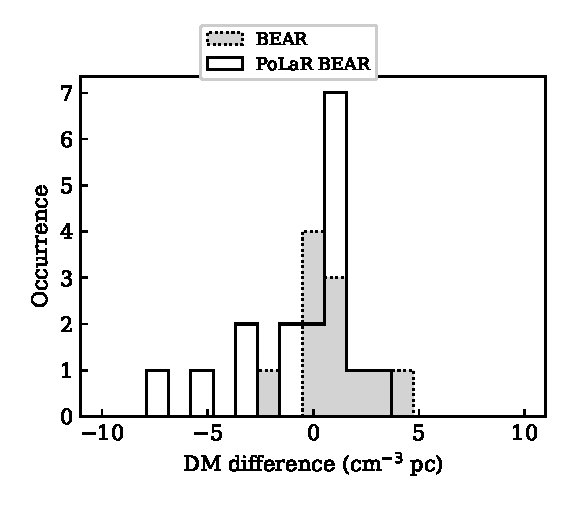
\includegraphics[width=\textwidth]{Graphs/frbdmdiff.eps}
    \end{minipage}%
    \begin{minipage}{0.5\textwidth}
        \includegraphics[width=\textwidth]{Graphs/fakedmdiff.eps}
    \end{minipage}
    \caption[Histograms of DM difference]{Histograms of DM difference in detections from PoLaR BEAR and BEAR for real FRB data (left) and fake FRB data (right).}
    \label{fig:dmdiff}
\end{figure}

\subsection{Detection W}

Histograms of the W difference in detections from PoLaR BEAR and BEAR for real FRB data and fake FRB data are shown in Figure \ref{fig:wdiff}. The outliers here are defined to be data with W difference of $\pm 10$ ms. For real FRB data, PoLaR BEAR exhibited no outliers whereas BEAR has 1 outlier ($1509$ ms). For fake FRB data, both PoLaR BEAR and BEAR exhibited no outliers, with most detections occuring within $\pm 2$ ms. It can be seen that for real FRBs, detections from BEAR do have smaller errors whereas PoLaR BEAR reports larger W. On the other hand, for fake FRBs, PoLaR BEAR was much more consistent with much more detections occuring close to the true W.

\begin{figure}
    \centering
    \begin{minipage}{0.5\textwidth}
        \includegraphics[width=\textwidth]{Graphs/frbwdiff.eps}
    \end{minipage}%
    \begin{minipage}{0.5\textwidth}
        \includegraphics[width=\textwidth]{Graphs/fakewdiff.eps}
    \end{minipage}
    \caption[Histograms of W difference]{Histograms of W difference in detections from PoLaR BEAR and BEAR for real FRB data (left) and fake FRB data (right).}
    \label{fig:wdiff}
\end{figure}

\subsection{Detection SNR}

Histograms of the SNR difference in detections from PoLaR BEAR and BEAR for real FRB data and fake FRB data are shown in Figure \ref{fig:snrdiff}. The outliers here are defined to be data with SNR difference of $\pm 30$. For real FRB data, PoLaR BEAR exhibited no outliers whereas BEAR has 1 outlier ($-49.32$). For fake FRB data, both PoLaR BEAR and BEAR exhibited no outliers, with most detections occuring within $\pm 10$. In both cases, PoLaR BEAR performs as well as BEAR. 

\begin{figure}
    \centering
    \begin{minipage}{0.5\textwidth}
        \includegraphics[width=\textwidth]{Graphs/frbsnrdiff.eps}
    \end{minipage}%
    \begin{minipage}{0.5\textwidth}
        \includegraphics[width=\textwidth]{Graphs/fakesnrdiff.eps}
    \end{minipage}
    \caption[Histograms of SNR difference]{Histograms of SNR difference in detections from PoLaR BEAR and BEAR for real FRB data (left) and fake FRB data (right).}
    \label{fig:snrdiff}
\end{figure}
\chapter{Discussions}\label{discuss}

\section{Performance Quantization}

To further quantify the performance of PoLaR BEAR, the average deviations in the detection parameters were observed. Table \ref{tab:frbdev} and \ref{tab:fakedev} shows the average deviations in the detections for PoLaR BEAR and BEAR for both real FRB data and fake FRB data respectively. For real FRB data, it can be see that PoLaR BEAR performs significantly better than BEAR for detection DM and W, and only slightly worse for detection SNR. For fake FRB data, it can be see that PoLaR BEAR performs slightly worse than BEAR for detection DM and SNR, and slightly better for detection SNR. Therefore, it can be confirmed that PoLaR BEAR performs comparably well with BEAR.

\begin{table}
\centering
\def\arraystretch{1.25}
\caption[Average deviations in the detection parameters for real FRB data]{Average deviations in the detection parameters using PoLaR BEAR and BEAR for real FRB data.}
\begin{tabular}{cccc}
\hline
Parameter & DM ($\cmp$) & W (ms) & SNR\\
\hline
PoLaR BEAR & 2.9953  & 1.6203   & 10.4972 \\
BEAR       & 45.9694 & 116.6431 & 9.9726  \\
\hline
\end{tabular}
\label{tab:frbdev}
\end{table}
\begin{table}
\centering
\def\arraystretch{1.25}
\caption[Average deviations in the detection parameters for fake FRB data]{Average deviations in the detection parameters using PoLaR BEAR and BEAR for fake FRB data.}
\begin{tabular}{cccc}
\hline
Parameter & DM ($\cmp$) & W (ms) & SNR\\
\hline
PoLaR BEAR & 2.0530   & 0.4282  & 5.0371 \\
BEAR       & 1.7404   & 0.5089  & 3.8685  \\
\hline
\end{tabular}
\label{tab:fakedev}
\end{table}

There was also one significant outlier for detections in BEAR that were not present in PoLaR BEAR, namely FRB 010724. BEAR detected a DM of $930.767 \cmp$, which is $555.767 \cmp$ away from the actual value, whereas PoLaR BEAR reported a DM of $374 \cmp$. BEAR also detected a W of $1529\,\text{ms}$, which is $1509\,\text{ms}$ away from the actual value, whereas PoLaR BEAR reported a W of $24\,\text{ms}$. Figure \ref{fig:frb010724} shows the candidate plot of the detection in PoLaR BEAR. A large decrease in flux after the burst can be seen due to saturation of the receiver, causing the inaccurate detection in BEAR. 

\begin{sidewaysfigure}
    \centering
    \includegraphics[width=0.9\textwidth]{Images/FRB010724.jpeg}
    \caption{PoLaR BEAR candidate output for FRB 010724.}
    \label{fig:frb010724}
\end{sidewaysfigure}

\section{Underestimation of SNR}

In general, the SNRs are detected by PoLaR BEAR and BEAR can be seen to be slightly lower than that of the true values. This is expected as inaccurate DM and W values when performing the calculation for $S$ would result in lower $S$ values, and consequently lower detected SNR. For a DM offset of $\delta$DM, the ratio between the SNR detected and the true SNR is \cite{Cordes2003}
\begin{equation}
    \frac{\text{SNR}}{\text{SNR}_0} = \frac{\sqrt{\pi}}{2} \zeta^{-1} \text{erf }\zeta
\end{equation}
where $\text{SNR}_0$ is the true SNR if the dedispersion is perform at the true DM. $\zeta$ is the ratio between the time delay caused by the DM offset and pulse width given by
\begin{equation}
    \zeta = 6.91 \times 10^{-3} \delta \text{DM} \frac{\Delta\nu_{\text{MHz}}}{W_{\text{ms}}\nu^3_{\text{GHz}}}
\end{equation}
As for a W offset of $\delta W$, the SNR ratio becomes \cite{Men2019}
\begin{equation}
    \frac{\text{SNR}}{\text{SNR}_0} = \begin{cases}\frac{W}{W+\delta W}, & \text{for }\delta W\geq 0, \\ \frac{W+\delta W}{W}, & \text{for }\delta W < 0\end{cases}
\end{equation}
For any non-zero offset in DM and W, both cases results a lower detection SNR compared to SNR$_0$, shown in Figure \ref{fig:snrdev}. 

\begin{figure}
    \centering
    \begin{minipage}{0.5\textwidth}
    \includegraphics[width=\textwidth]{Graphs/snrdm.eps}
    \end{minipage}%
    \begin{minipage}{0.5\textwidth}
    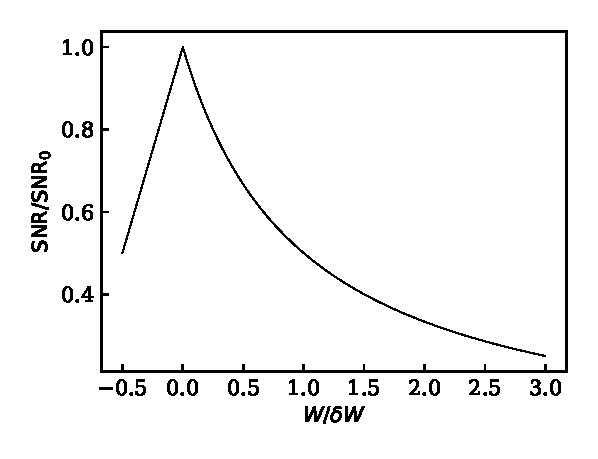
\includegraphics[width=\textwidth]{Graphs/snrw.eps}
    \end{minipage}
    \caption[SNR deviation due to DM and W offset]{Graph of SNR deviation due to DM offset i.e. $\zeta \propto \delta\text{DM}$ (left), and due to W offset i.e. $\delta W/W$ (right). Detected SNR decreases for any non-zero $\delta\text{DM}$ and $\delta W/W$.}
    \label{fig:snrdev}
\end{figure}

\section{Differences between PoLaR BEAR and BEAR}

Other than the differences between Python and C++, there are two main differences between PoLaR BEAR and BEAR. The first is the division of trial DMs. In BEAR, subband dedispersion is use to improve its efficacy \cite{Barsdell2012}. Subband dedispersion is an approximation approach in reducing the computation cost of dedispersion. The process involves splitting up the DM range into several subranges, each centered around a nominal DM value. The frequency channels are also partitioned into subbands. The delays for every nominal DMs are subtracted from the subbands, resulting in partially dedispersed subbands. The data is then passed through the usual dedispersion at the remaining DMs. This results in a trial DM array with differing increments depending on the nominal DM, usually larger increments at higher DMs, as shown in Table \ref{tab:subband} \cite{Magro2011}.

\begin{table}[h]
    \def\arraystretch{1.25}
    \caption[Example of a subband dedispersion plan]{Example of a subband dedispersion plan for a pulsar survey. $\Delta$Sub$_{\text{DM}}$ refers to the DM step between two successive nomial DM values, $\Delta$DM is the finer step used for creating the dedispersed time series around a particular nominal DM value.}
    \centering
    \begin{tabular}{ccccc}
        \hline
        Pass & Low DM & High DM & $\Delta$DM & $\Delta$Sub$_{\text{DM}}$ \\
        & ($\cmp$) & ($\cmp$) & ($\cmp$) & ($\cmp$) \\
        \hline
        1 & 0.00 & 53.46 & 0.03 & 0.66 \\
        2 & 53.46 & 88.26 & 0.05 & 1.2 \\
        3 & 88.26 & 150.66 & 0.10 & 2.4 \\
        \hline
    \end{tabular}
    \label{tab:subband}
\end{table}

However, in PoLaR BEAR, I opted to set the DM range and a single increment in the beginning (usually from 1 to 2000 $\cmp$ with increments of 1 $\cmp$) and use the usual brute force dedispersion. This is because the program is aimed to allow for an easier understanding in FRB detection instead of performance. 

Another difference is in the definition of the detection time or also known as the pulse epoch, $t_0$. In BEAR, $t_0$ is defined to be the beginning of the pulse, allowing it to utilize efficient looping methods for the calculation of $S$. However in PoLaR BEAR, $t_0$ is defined to be in the middle of the pulse, allowing the usage of convolution in the program which follows the usual Python style. 

\section{GPU Dedispersion}

As stated in \citeNP{Magro2011}, graphics processing unit or GPU computation can also speed up dedispersion to improve real time detection of radio transients. Using NVIDIA's CUDA cores, dedispersion can be parallelized over many GPU threads, simultaneously operating on many different DMs. Tests have shown that GPUs speed up dedispersion by 50 to 200 times \cite{Magro2011} or at least by 9 times \cite{Barsdell2012} when compared to single-threaded CPU implementation. This is applied in many FRB searches e.g. AMBER used on the Westerbork Telescope \cite{Sclocco2020} and the Medicina BEST-2 transient search pipeline \cite{MAGRO2013}. 

In Python, two packages allows python to utilize GPU to speed up numpy functions, namely \texttt{CuPy} and \texttt{Numba}. In this case, \texttt{CuPy} was used as it is a more complete reimplementation of \texttt{Numpy} using the GPU, compared to \texttt{Numba} where custom algorithms tailored to its format is required \cite{Okuta2017}.

To test the performance increase of GPU dedispersion in this case, the data was generated using the same method with the same properties as for fake FRB, with varying observation times i.e. 0.125, 0.25, 0.5, 1, 2, and 5 minutes, and varying number of frequency channels i.e. 128, 256, 512, and 1024 frequency channels. The data is also downsampled by 20 to reduce computation time. The data is then dedispersed using both brute force dedispersion with \texttt{numpy.roll} and a modified dedispersion with \texttt{cupy.roll} at a single DM (1000$\cmp$), as dedispersion at different DMs should not affect the performance significantly. Note that the GPU used here is the GTX 1660 Ti, with 1536 CUDA cores rated at a maximum of 169.9 GFLOPS, and 6 GB of memory. 

Figure \ref{fig:gpu} shows the graph of the speed-up factor of GPU dedispersion compared to the brute force CPU implementation for different data length/observation time, as well as at different number of frequency channels. The speed-up factor can be seen to increase with observation times up to a factor of 8, but shorter observation times result in speed-up factors of less than one i.e. GPU dedispersion slower than CPU implementation, which could be due to the memory transfer latency between the RAM and the GPU memory. Therefore, implementation of GPU dedispersion in PoLaR BEAR using \texttt{CuPy} can be beneficial to improve its performance. Note that the benefits may scale further at larger observation time, but requires a much larger amount of GPU memory, which is the reason that the tests was only done for data up to 5 minutes observation time with 1024 frequency channels. 

\begin{figure}
    \centering
    \includegraphics[width=0.7\textwidth]{Graphs/gpu.eps}
    \caption[Speed-up factor for GPU dedispersion]{Graph of speed-up factor between GPU dedispersion and usual CPU dedispersion for different data lengths and different number of frequency channels.}
    \label{fig:gpu}
\end{figure}

% However, upon implementation of CuPy on PoLaR BEAR, we noticed that the program took much longer times to analyze the data. This can be due to:
% \begin{enumerate}
%     \item Memory transfer latency between the RAM and GPU for non-CuPy functions. Certain functions like the numpy.add.reduceat are not available in CuPy, resulting us to copy the data back and forth from the GPU to the RAM and back to the GPU. This latency would accumulate, resulting in the program running much slower.
%     \item Limited GPU memory. Large amounts of data may bottleneck the GPU memory, causing some buffer to be stored in the RAM instead, resulting in the same issue as stated earlier.
%     \item Short observation period. To reduce memory usage in the GPU as stated before, the data is cut to short observation times. As we have seen, this can cause the GPU dedispersion to be slower than the usual dedispersion, again due to memory transfer latency.
% \end{enumerate}
% Therefore, we decided to maintain the usual dedispersion in PoLaR BEAR.

%Comsumer GPUs have little memory compared to workspace GPUs e.g. quadro
\chapter{Summary}\label{summary}

FRBs are bright, broadband radio emission ranging from milliseconds or less. The key characteristic of FRBs is their dispersion measure or DM, seen as a frequency-dependent delay in the signal. Most FRBs have DMs more than the contribution from our galaxy, suggesting its extragalactic nature. The signal characteristics seem to suggest that FRBs come from magnetars. FRBs are usually detected using single-dish telescopes, and the data is passed through pipelines that perform the detection and analysis of the FRBs. 

% As stated earlier, the objectives of this project are to understand FRB detection methods, which is mainly based on the likelihood statistic ratio, to develop a program that independently searches for FRBs in radio telescope data, for which I developed PoLaR BEAR, to compare its performance with BEAR, where its performance can be seen to the comparable, and to test the performance increase for GPU dedispersion, for which \texttt{CuPy} can be seen to provide up to 8 times speedup for dedispersion.

% Here, I created the PoLaR BEAR independent FRB detection program that searches of FRBs in radio telescope data in Python, based on BEAR. The program involves many functions, where the three main ones are RFI mitigation, dedispersion, and matched filtering. RFI mitigation is performed by zapping frequency channels with RFI, and by using ZDMF to remove any narrow-band short-duration RFI with no dispersive nature. Dedispersion shifts the data to compensate for the dispersion to maximize the SNR of the FRB. Matched filtering then calculates the SNR in the data based on the likelihood statistic ratio for all DM, time, and W, then peaks in the SNR denotes an FRB detection. 

% PoLaR BEAR is tested with real FRB data and fake FRB data generated using Python. PoLaR BEAR performs well with small deviations in the detection parameters compared to the actual parameters, comparable to that of BEAR. The detection SNR are also slightly underestimated as expected due to deviations in DM and W. GPU dedispersion was also tested in PoLaR BEAR using \texttt{CuPy}, and the process can be sped up by up to 8 times compared to brute force dedispersion. 

% With this, an independent FRB detection pipeline was successfully created using Python. Detecting more FRBs will help in pinpointing the correct origin of FRBs. If they are from magnetars, FRBs would be a crucial way to study their properties e.g. the origin of their strong magnetic fields, their composition, their formation origin, and the types of stars that would transition into them.

The first objective of this project was to understand FRB detection methods, which are mainly done using matched filtering and the likelihood statistic ratio. 

The second objective was to develop a program that independently searches for FRBs in radio telescope data. Here, I created the PoLaR BEAR independent FRB detection program that searches of FRBs in radio telescope data in Python, based on BEAR. The program involves many functions, where the three main ones are RFI mitigation, dedispersion, and matched filtering. RFI mitigation is performed by zapping frequency channels with RFI, and by using ZDMF to remove any narrow-band short-duration RFI with no dispersive nature. Dedispersion shifts the data to compensate for the dispersion to maximize the SNR of the FRB. Matched filtering then calculates the SNR in the data based on the likelihood statistic ratio for all DM, time, and W, then peaks in the SNR denotes an FRB detection. 

The third objective was to compare the performance of the program developed with BEAR. PoLaR BEAR was tested with real FRB data and fake FRB data generated using Python. PoLaR BEAR performs well with small deviations in the detection parameters compared to the actual parameters, comparable to that of BEAR. The detection SNR are also slightly underestimated as expected due to deviations in DM and W.

The final objective was to test the performance increase for GPU dedispersion. In this case, GPU dedispersion was implemented in PoLar BEAR using \texttt{CuPy}, and dedispersion can be sped up by up to 8 times compared to brute force CPU dedispersion.

With this, an independent FRB detection pipeline was successfully created using Python. Detecting more FRBs will help in pinpointing the correct origin of FRBs. If they are from magnetars, FRBs would be a crucial way to study their properties e.g. the origin of their strong magnetic fields, their composition, their formation origin, and the types of stars that would transition into them.

\bibliography{ref}

%\begin{appendices}
\chapter{PoLaR BEAR Example Output}\label{app:polarbear}
Shown here are PoLaR BEAR outputs for FRB 110220. Main analysis plot in Figure \ref{fig:main} consists of (a) filterbank data, (b) frequency profile of first candidate, (c) integrated frequency profile of first candidate, (d) S as a function of DM and time, (e) S as a function time, (f) pulse profile of first candidate, (g) S as a function of W and DM, (h) S as a function of W, and (i) S as a function of DM. Candidates' pulse profile plots is shown in Figure \ref{fig:prof}. Candidates' analysis plot in Figure \ref{fig:cand} consists of (a) pulse profile of the candidate, (b) dedispersed filterbank data, (c) frequency profile of the candidate, (d) integrated frequency profile of the candidate, (e) S as a function of DM and time, (f) S as function of DM, (g) S as a function of time, (h) S as a function of W and DM, (i) S as a function of W, and (j) S as a function of DM. Analysis properties and results is shown in Figure \ref{fig:prop}.

\begin{figure}
    \centering
    \includegraphics[width=\textwidth]{Images/Example/main.png}
    \caption[Example PoLaR BEAR main analysis plot]{Example PoLaR BEAR main analysis plot for FRB 110220.}
    \label{fig:main}
\end{figure}

\begin{figure}
    \centering
    \includegraphics[width=\textwidth]{Images/Example/profile.jpeg}
    \caption[Example PoLaR BEAR candidates' pulse profile plots]{Example PoLaR BEAR candidates' pulse profile plots for FRB 110220.}
    \label{fig:prof}
\end{figure}

\begin{sidewaysfigure}
    \centering
    \includegraphics[width=0.9\textwidth]{Images/Example/cand.png}
    \caption[Example PoLaR BEAR candidates' analysis plot]{Example PoLaR BEAR candidates' analysis plot for FRB 110220.}
    \label{fig:cand}
\end{sidewaysfigure}

\begin{figure}
    \centering
    \includegraphics[width=\textwidth]{Images/Example/prop.jpg}
    \caption[Example PoLaR BEAR analysis properties and results]{Example PoLaR BEAR analysis properties and results for FRB 110220.}
    \label{fig:prop}
\end{figure}
\end{appendices}

\end{document}